% -*-latex-*-
% Filename: viewer.tex
% Author: Rob MacLeod and Dave Weinstein
%
% Last update: Fri Feb 23 15:51:37 2001 by Rob MacLeod
%    - created
%
%%%%%%%%%%%%%%%%%%%%%%%%%%%%%%%%%%%%%%%%%%%%%%%%%%%%%%%%%%%%%%%%%%%%%%
%%%%%%%%%%  Figures used in this file %%%%%%%%%%%%%%%%%%%%%%%%%%%%%%%%
%begin{latexonly}
  \newcommand{\viewerwindow}%
  {\centerline{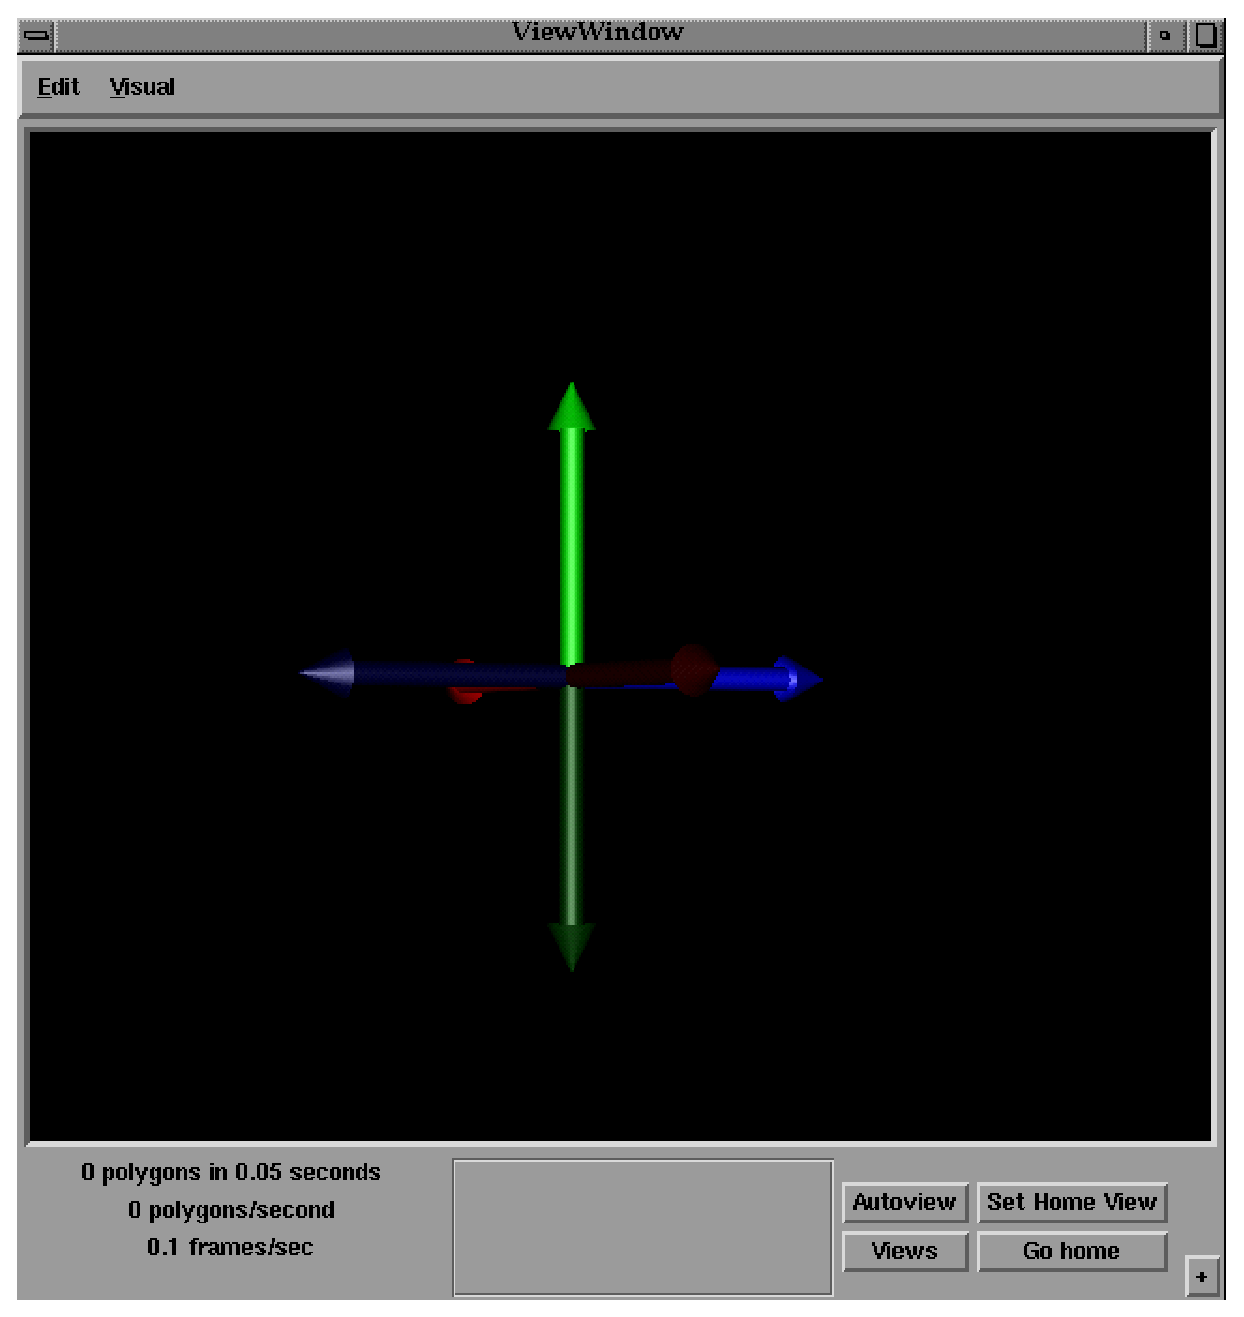
\epsfig{file=figures/viewwindow.eps,width=\columnwidth}}}
%end{latexonly}
\begin{htmlonly}
  \newcommand{\viewerwindow}{%
  \htmladdimg[align=top,width=8,alt="module"]
  {../figures/viewwindow.gif}}
\end{htmlonly}

%begin{latexonly}
  \newcommand{\extendedwindow}%
  {\centerline{\epsfig{file=figures/ext-viewwindow.eps,width=\columnwidth}}}
%end{latexonly}
\begin{htmlonly}
  \newcommand{\extendedwindow}{%
  \htmladdimg[align=top,width=8,alt="module"]
  {../figures/ext-viewwindow.gif}}
\end{htmlonly}
%%%%%%%%%%%%%%%%%%%%%%%%%%%%%%%%%%%%%%%%%%%%%%%%%%%%%%%%%%%%%%%%%%%%%%
\newcommand{\viewer}{\emph{Viewer}}
\newcommand{\graphics}{\emph{Graphics}}

\section{Visualization with the \viewer{}}
\label{sec:viewerer}

This section describes perhaps the most frequently used module of \SR{},
the \viewer{}, which has the task of displaying interactive graphical output
to the computer screen.  You will use the \viewer{} any time you wish to see
a geometry, some spatial data.  More important for the computational
steering (described in Section~\ref{sec:con-steering}), is that the \viewer{}
provides access to many simulation parameters and controls and thus
indirectly initiates new iterations of the simulation steps.

We begin with an overview of the \viewer{} window and its controls, then
describe in detail all the options and variations.

\subsection{Anatomy of the \viewer{} window}
\label{sec:viewer-anatomy} 

The \viewer{} window contains two main areas, the upper portion, called the
\graphics{} window, which displays the graphics, and the lower portion,
where most of the control buttons are.  Figure~\ref{fig:viewwindow}
contains an example of a \viewer{} window. In the \graphics{}
window, control is mostly by means of the mouse, mouse buttons, and various
modifier keys (shift/control/alt).  In the lower window are a lot of
buttons and sliders, the function of which will become clear when you read
this manual.

\begin{figure}[htb]
  \begin{makeimage}
  \end{makeimage}
%  \viewerwindow
    \framebox{\parbox[3in]{\columnwidth}{The\dotfill Figure\\
    \vspace{2in}\\
    With some \dotfill dummy text}}
  \caption{\label{fig:viewwindow} The default \viewer{} window in \SR{}}
\end{figure}


First, try out the controls for the \graphics{} window by moving the mouse
to the center of the viewer window and clicking and holding the left button
and then dragging the mouse.  The objects should translate along with the
mouse.  Do the same operation with the middle mouse button and the objects
will rotate around a point in the center of the display.  The right mouse
button controls the scale of the display, zooming in  when the mouse moves
downward or to the right.  See Section~\ref{sec:view-mouse} for all the
gory details on mouse control.

The control visible along the bottom of the \viewer{} window set some basic
configurations as follows:
%
\begin{description}
  \item [Autoview: ] restores the display back to a default condition, very
        useful when some combination of settings results in the objects
        disappearing from the view window.
  \item [Set Home View: ] captures the setting of the current view so you
        can return to it later by clicking the ``Go home'' button.
  \item [Go home: ] restore the current home view.
  \item [Views: ] lists a number of standard viewing angles and
        orientations.  The view directions align with the Cartesian axes
        of the objects and the ``Up vector'' choice sets the orientation of
        the objects when viewed along the selected axis.
\end{description}

In the left corner of the control panel of the \viewer{} window are
performance indicators that document the current rendering speed for the
display.  The better the workstation you have, the higher the drawing rate.

In the lower right corner of the \viewer{} window is a small plus sign
(``+'').  Clicking on this reveals the extended control panel with controls
that we will describe in detail in Section~\ref{sec:view-control}.



\subsubsection{Menus}

At the top of the \viewer{} window are to pull-down menus.
\begin{description}
  \item [Edit: ] provides access to controls for the background color for
        the window as well as the clipping planes (requires the ``Use
        Clip'' control to be selected in the extended controls described in
        Section~\ref{sec:view-control}.
  \item [Visual: ] allows you to select between different graphics hardware
        settings available.  The list is ordered from most to least
        appropriate for the actual workstation hardware.
\end{description}

\subsection{Mouse control in the \viewer{} window}
\label{sec:view-mouse} 

The mouse controls within \SR{} and extensive and flexible, depending on
the mouse button, any simultaneous control keys, and the way the mouse
moves.  The description below may seem overly complicated at first, but
with a little playing, it becomes intuitive (another way of saying you will
learn it if you use it enough).

\begin{center}
  \begin{tabular}{|l|l|p{3in}|} \hline
    \multicolumn{3}{|c|}{Mouse Controls}\\
    \multicolumn{1}{|c|}{Control Key} & 
    \multicolumn{1}{|c|}{Button} & 
    \multicolumn{1}{|c|}{Action}\\ \hline
None & Left & translate objects \\
     & Middle & rotate objects about the center of the scene on an arc ball
    that surrounds the object; rotation direction is a function of the
    initial mouse location so try different sites and note response. \\ 
     & Right & zoom or scale objects (downwards and to the right increases
     size, upwards or to the left decreases size) \\ 
     & Right & activate pull-down menu \\ \hline
Shift & Left & select an object or a widget in the display \\
      & Middle &  no action \\
      & Right &  no action \\ \hline
Control & Left & translate in the Z-direction, \ie{} in and out of the
    screen (down moves closer, up further away).  If the cursor is over a
    point in an object when clicked, this point becomes the center of the
    screen for translation.\\ 
      & Right & Unicam movement (see next table)\\ \hline
\end{tabular}

\bigskip

\begin{tabular}{|l|p{3in}} \hline
    \multicolumn{2}{|c|}{Effect of Control key} \\ \hline
    \multicolumn{1}{|c|}{Initial movement} & 
    \multicolumn{1}{|c|}{Action}\\ 
    \hline
    \multicolumn{2}{|c|}{Left mouse button (Dolly movement)}\\
    Horizontal & change acceleration of zoom (right increases) \\
    Vertical & zoom in (down) and out (up) at fixed acceleration \\
    None & selects the look at point that we then zoom toward \\
    \hline
    \multicolumn{2}{|c|}{Panning (Middle mouse button)} \\
    All  & rotate the lookat point about the eye location \\
    \hline
    \multicolumn{2}{|c|}{Unicam Behavior (Control-Right Mouse}\\
    \multicolumn{1}{|c|}{Initial mouse location} & 
    \multicolumn{1}{|c|}{Action}\\ 
    \hline
    Near edge of display & rotate objects on the arc ball \\
    Near the objects & following behavior: \\
    \hline
    \multicolumn{1}{|c|}{Initial mouse movement} & 
    \multicolumn{1}{|c|}{Action}\\ 
    Horizontal & pan objects \\ 
    Vertical & zoom and pan: down = zoom in, up = zoom
    out, left and right= pan left and right) \\
    None & sets rotation point for subsequent arc ball rotation.\\

\end{tabular}
\end{center}


\subsection{Extended control window}
\label{sec:view-control} 

Clicking on the ``+'' sign in the lower right corner of the default
\viewer{} window and the window expands to reveal an extended panel of
control buttons, as shown in Figure~\ref{fig:extviewwindow}.  Click on the
``-'' sign that now replaces the ``+'' and this extended panel disappears
again.  Here we describe the control options available in the extended
control window.

\begin{figure}[htb]
  \begin{makeimage}
  \end{makeimage}
%  \extendedwindow
    \framebox{\parbox[3in]{\columnwidth}{The\dotfill Figure\\
    \vspace{2in}\\
    With some \dotfill dummy text}}
  \caption{\label{fig:extviewwindow} The lower portion of extended
    \viewer{} window in \SR{}} 
\end{figure}


\subsubsection{Object selector}

The lower portion of the extended \viewer{} window is divided into three
columns and the middle of these contains a list of all the objects in the
display.  If the list becomes long enough, a scroll bar control on the left
hand side controls which are visible.  For each entry in the list, we have
the following controls, reading from left to right:

\begin{itemize}
  \item At the left end of each of the
        objects in the list, there is box that displays red when it is
        selected.  The \viewer{} window only displays those objects that
        are selected.
  \item Next comes the name of the object.
  \item The control box that comes next determines the type of lighting in
        effect for the object.  Choices include ??.
  \item As the right end of each entry is the ?? control.
\end{itemize}

Clicking on an entry in the list selects that object for all the rendering
controls described in the next section.

\subsubsection{Rendering controls}

The left column of the  extended \viewer{} window contains controls that
apply to all the selected objects in the display.  If no object is
selected, than rendering changes apply to all visible surfaces.  Selecting
one or more surfaces
%?? Can we select multiple surfaces??
causes all changes to act on only the selected surface(s).  The individual
controls are all toggles that switch the following actions:
\begin{description}
  \item [Lighting: ] toggle whether the \viewer{} applies lighting to the
        display. 
  \item [Fog: ] fog is also known as ``depth cueing'' and draws objects
        with different intensity based on their distance from the user.
        Close object appear brighter while distant objects fade graduate
        into the background as a function of distance from the front. 
  \item [BBox: ] selecting the control displays a box in the display that
        contains all the objects 
%?? both visible and invisible ones??
  \item [Use Clip: ] apply up to six clipping planes to the display
%?? how does this work??
  \item [Back Cull: ] display only the forward facing facets of any surface
        objects in the display.
  \item [Display List: ]
%?? what does this do??
  \item [Shading: ] select the type of shading for the objects with
        surfaces in the display about the following options:
        \begin{description}
          \item [Wire: ] show only the wire mesh of objects.
          \item [Flat: ] draw each facet with a constant color.
          \item [Gouraud: ] linearly interpolate the color across facets. 
        \end{description}
\end{description}

The right hand column of the extended \viewer{} window contains controls
for displaying the axes and creating stereoscopic rendering.  

\paragraph{Stereo viewing: } requires hardware LCD glasses synchronized
with the display so that visibility for each eye is synchronized with the
display of the appropriate view.  The ``Fusion Scale'' control provides a
means of setting the eye separation and thus setting the view that is most
suited to facial anatomy and distance from the screen.

%?? More detail on the stereo viewing models

\subsubsection{Making movies}
\label{sec:view-movies} 

The \viewer{} window in \SR{} has simple controls for capturing sequences
of images into animations or movies.  Here we describe how this works.

In the left column of the extended \viewer{} window are controls for
selecting movie type and then initiating and stopping the acquisition of
individual frames in the movie.

%?? More details on how this works.